%!TEX program = pdflatex
\documentclass[UTF8]{article}

\usepackage[UTF8]{ctex}
\usepackage{amsmath}
\usepackage{enumerate}
\usepackage{amssymb}
\usepackage{graphicx}
 
\title{Homework 11.02}
\author{SA18225036 陈旻}
\date{}
    \begin{document}
    \maketitle
    \section{Question 39}
    \paragraph{Question}
    Determine the number of solutions of the equation $ x_{1} + x_{2} + x_{3} + x_{4} = 14 $ in nonnegative integers $ x_{1} $, $ x_{2} $, $ x_{3} $, and $ x_{4} $ not exceeding 8.
    \paragraph{Answer}
    \begin{center}
        
    \end{center}

    \section{Question 40}
    \paragraph{Question}
    At a party seven gentlemen check their hats. In how many ways can their hats be returned so that
    \begin{enumerate}[(a)]
    \item no gentleman receives his own hat?
    \item at least one of the gentlemen receives his own hat?
    \item at least two of the gentlemen receive their own hats?
    \end{enumerate}
    \paragraph{Answer}
    \begin{center}
    \end{center}

    \section{Question 41}
    \paragraph{Question}
    What is the number of ways to place six nonattacking rooks on the 6-by-6 boards with forbidden positions as shown?
    \begin{figure}[ht]
        \centering
        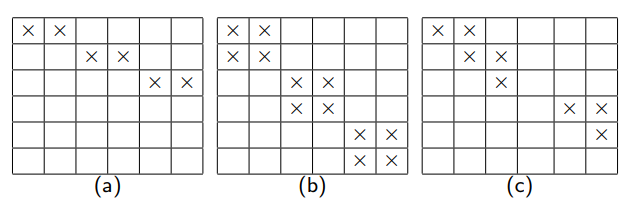
\includegraphics[scale=0.6]{img/t41.png}
        \end{figure}
    
    \paragraph{Answer}
    \begin{center}
    \end{center}

    \section{Question 42}
    \paragraph{Question}
    A carousel has eight seats, each representing a different animal. Eight girls are seated on the carousel facing forward (each girl looks at another girl’s back). In how many ways can they change seats so that each has a different girl in front of her? How does the problem change if all the seats are identical?
    \paragraph{Answer}
    \begin{center}
    \end{center}

    \section{Question 44}
    \paragraph{Question}
    Prove the following about the Fibonacci numbers,
    \begin{enumerate}[(a)]
        \item $ f_{n} $ is even if and only if n is divisible by 3.
        \item $ f_{n} $ is divisible by 3 if and only if n is divisible by 4.
        \item $ f_{n} $ is divisible by 4 if and only if n is divisible by 6.
    \end{enumerate}
    \paragraph{Answer}
    \begin{center}
    \end{center}
    \end{document}